\documentclass[]{article}
\usepackage{etex}
\usepackage[margin = 1.5in]{geometry}
\setlength{\parindent}{0in}
\usepackage{amsmath}
\usepackage{amsfonts}
\usepackage{amssymb}
\usepackage{amsthm}
\usepackage{listings}
\usepackage{color}
\usepackage{mathtools}
\usepackage{multicol}
\usepackage[lined]{algorithm2e}
\usepackage{float}
\usepackage[T1]{fontenc}
\usepackage{ae,aecompl}
\usepackage[pdftex,
  pdfauthor={Michael Noukhovitch},
  pdftitle={COMP767},
  pdfsubject={Lecture notes from Doina Precup},
  pdfproducer={LaTeX},
  pdfcreator={pdflatex}]{hyperref}
\usepackage{graphicx}
\usepackage{cleveref}
\usepackage{enumitem}

\definecolor{dkgreen}{rgb}{0,0.6,0}
\definecolor{gray}{rgb}{0.5,0.5,0.5}
\definecolor{mauve}{rgb}{0.58,0,0.82}

\lstset{
  language=C,
  aboveskip=3mm,
  belowskip=3mm,
  showstringspaces=false,
  columns=flexible,
  basicstyle={\small\ttfamily},
  numbers=none,
  numberstyle=\tiny\color{gray},
  keywordstyle=\color{blue},
  commentstyle=\color{dkgreen},
  stringstyle=\color{mauve},
  breaklines=true,
  breakatwhitespace=true,
  tabsize=4
}

\theoremstyle{definition}
\newtheorem*{defn}{Definition}
\newtheorem{ex}{Example}[section]
\newtheorem*{theorem}{Theorem}

\setlength{\marginparwidth}{1.5in}
\setlength{\algomargin}{0.75em}

\DeclarePairedDelimiter{\set}{\lbrace}{\rbrace}

\definecolor{darkish-blue}{RGB}{25,103,185}

\usepackage{hyperref}
\hypersetup{
    colorlinks,
    citecolor=darkish-blue,
    filecolor=darkish-blue,
    linkcolor=darkish-blue,
    urlcolor=darkish-blue
}
\newcommand{\lecture}[1]{\marginpar{{\footnotesize $\leftarrow$ \underline{#1}}}}
\newcommand{\N}{\mathbb{N}}
\newcommand{\Z}{\mathbb{Z}}
\newcommand{\E}{\mathbb{E}}
\newcommand{\Lagr}{\mathcal{L}}
\DeclareMathOperator*{\argmin}{argmin}
\DeclareMathOperator*{\argmax}{argmax}

\makeatletter
\def\blfootnote{\gdef\@thefnmark{}\@footnotetext}
\makeatother

\graphicspath{{./comp767/}}

\begin{document}
\let\ref\Cref

\title{\bf{COMP767: Reinforcement Learning}}
\date{Winter 2018, \\ \center Notes written from Doina Precup's lectures.}
\author{Michael Noukhovitch}

\maketitle
\newpage
\tableofcontents
\newpage

\section{Introduction}
\label{sec:introduction}

\subsection{Definitions}
\label{sub:definitions}
Reinforcement learning is:
\begin{description}
    \item[agent-oriented learning] learning by interacting with an environment
    \item[trial and error] only given delayed evaluative feedback
    \item[science of the mind] one which is neither natural science nor applied technology
\end{description}

Framework:
\begin{enumerate}
    \item agent percieves the \textbf{state} of the environment
    \item based on the state, it chooses an \textbf{action}
    \item the action gives the agent a \textbf{reward}
    \item a \textbf{policy} aims to maximize the agent's \textbf{long term expected reward}
\end{enumerate}


\subsection{Key Factors of RL}
\label{sub:key_factors_of_rl}
\begin{itemize}
    \item trial and error search
    \item environment is stochastic
    \item reward may be delayed
    \item balancing exploration and exploitation
\end{itemize}

\subsection{Classical Challenges}
\label{sub:classical_challenges}
\begin{itemize}
    \item reward
    \item information is sequential
    \item delayed consequences
    \item balancing exploration/exploitation
    \item non-stationarity
    \item fleeting nature of time and online data
\end{itemize}


\section{Bandit}
\label{sec:bandit}

\subsection{Single-Armed Bandit}
\label{ssub:single_armed_bandit}
Simplest RL problem
\begin{itemize}
    \item pull the lever
    \item get some reward
    \item choose the best lever!
\end{itemize}

\subsection{k-armed Bandit}
\label{ssub:k_armed_bandit}
\begin{itemize}
    \item at every time step $t$, choose an action $A_t$ from $k$ possibilties
    \item recieve a reward $R_t$ dependent only on the action taken (i.i.d)
    \item $q_*(a) = \E [R_t | A_t = a], \medskip \forall a \in {1, \ldots k }$
\end{itemize}

\subsubsection{$\varepsilon$-Greedy Action Selection}
\label{ssub:explot}
Solve exploration/exploitation by usually selecting exploit (best action so far), but exploring (random action) with probability $\varepsilon$

\begin{figure}[ht]
    \centering
    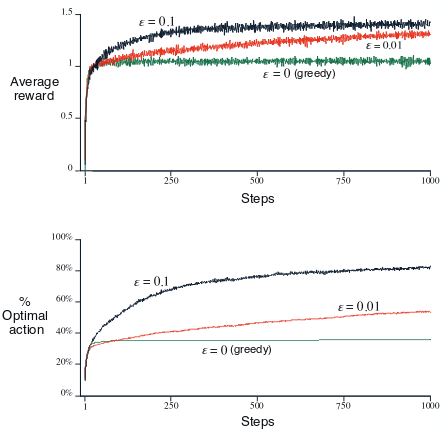
\includegraphics[width=0.5\linewidth]{epsilon_10arm.png}
    \caption{$\epsilon$-greedy methods on 10-arm bandit}
    \label{fig:}
\end{figure}


\subsection{Learning Rules}
\label{sub:learning_rules}

Learn the best policy by learning the reward for an action

\subsubsection{Averaging}
\label{ssub:averaging}

For a single action, update the new estimate based on old estimate and step size ($\alpha$), with all actions being equal
\begin{equation*}
    Q_{n+1} = Q_n + \alpha (R_n - Q_n)
\end{equation*}

\subsubsection{Recency-Weighted Average}
\label{ssub:recency_weighted_average}

\begin{description}
    \item[non-stationary] if the true action values change slowly over time
\end{description}

if so, then we need to put more weight on recent samples (using exponential)
\begin{equation*}
    Q_{n+1} = (1 - \alpha)^n Q_1 + \sum_{i=1}^n \alpha(1 - \alpha)^{n - i} R_i
\end{equation*}

\subsubsection{Optimistic}
\label{ssub:optimistic}
Previously we assumed $Q_1(a) = 0$, but we can start optimistically (e.g. $Q_1(a) = 5$) to encourage early exploration

\subsubsection{Upper Confidence Bound}
\label{ssub:upper_confidence_bound}
Reduce exploration over time after starting confident
\begin{itemize}
    \item estimate upper bound on true action values
    \item select the action with the largest upper bound
\end{itemize}

\begin{equation*}
    A_t = \argmax_a [Q_t(a) + c \sqrt{\frac{\log t}{N_t(a)}}]
\end{equation*}

\subsection{Evaluations}
\label{sub:evaluations}
\begin{description}
    \item[regret] the difference between best option and the one we chose $\max_a q_*(a) - q_t(a)$
    \item[expected total regret] $\E[\sum_t $ regret$_t]$ (optimal for UCB, Thomson sampling)
    \item[best response] regret for $T$ experimental trials after policy is fixed
\end{description}


\subsection{Gradient-Bandit Algorithms}
\label{sub:gradient_bandit_algorithms}

Don't need to learn specific rewards, just learn the \textbf{preference} $H_t(a)$, and try and make the probability of choosing an action $\pi_t(a)$ be proportional to it.

\begin{eqnarray*}
    \pi_t(a) &\propto e^{H_t(a)} \\
             &= \frac{e^{H_t(a)}}{\sum_b e^{H_t(b)}}
\end{eqnarray*}

if the reward for an action is better than average, increase its preference
\begin{eqnarray*}
    H_{t+1} &= H_t(a) + \alpha(R_t - \bar R_t)(1_{a = A_t} - \pi_t(a)) \\
\end{eqnarray*}
where $\bar R_t = $ average $R_i$

\subsection{Conclusions}
\label{sub:conclusions}
\begin{itemize}
    \item simple methods that can be built on
    \item learn from feedback
    \item appear to have a goal
\end{itemize}

\begin{figure}[ht]
    \centering
    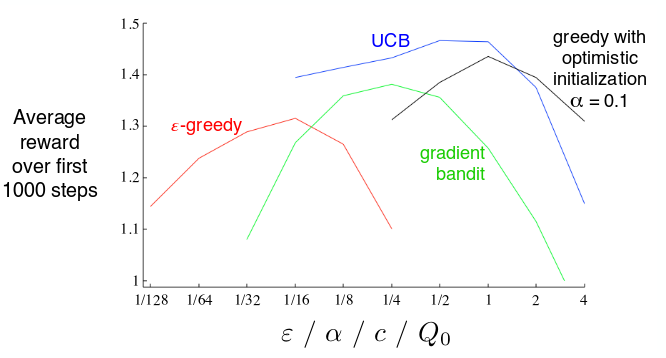
\includegraphics[width=0.7\linewidth]{bandit_comparison.png}
    \caption{bandit algorithm comparison}
    \label{fig:bandit-comparison}
\end{figure}


\end{document}
